\documentclass[a4,paper,fleqn]{article}

\usepackage{layout}

\DeclareSIUnit\year{Jahr}

\title{Notizen EEV -- SW05}
\date{\today}
\author{Daniel Winz}

\begin{document}
\maketitle
\clearpage

\section{Dynamik Triebwassersystem}

\subsection{Druckstoss}
Ursache: Beschleunigung negativ / positiv
\[ m \cdot a = m \frac{dv}{dt} \]

\subsection{Elastische Schwingungen}
Ursache: Elastizität Druckleitung, Kompressibilität Wasser

\subsection{Schwerkraft Schwingungen}
Ursache: Massenträgheit Wasserschloss

\section{Strömungslehre}

\subsection{Kontinuitätsgleichung}
\begin{figure}[h!]
    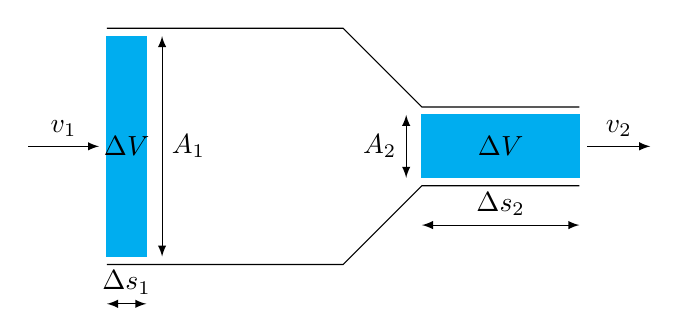
\begin{tikzpicture}
        \draw (0,0) -- (3,0) -- (4,1) -- (6,1);
        \draw (0,3) -- (3,3) -- (4,2) -- (6,2);
        \draw[cyan, fill=cyan] (0.0,0.1) rectangle node[black] {$\Delta V$} (0.5,2.9);
        \draw[cyan, fill=cyan] (4.0,1.1) rectangle node[black] {$\Delta V$} (6.0,1.9);
        \draw[latex-latex] (0.7,0.1) -- node[right] {$A_1$} (0.7,2.9);
        \draw[latex-latex] (3.8,1.1) -- node[left]  {$A_2$} (3.8,1.9);
        \draw[-latex] (-1,1.5) -- node[above] {$v_1$} (-0.1,1.5);
        \draw[-latex] (6.1,1.5) -- node[above] {$v_2$} (6.9,1.5);
        \draw[latex-latex] (0,-0.5) -- node[above] {$\Delta s_1$} (0.5,-0.5);
        \draw[latex-latex] (4.0,0.5) -- node[above] {$\Delta s_2$} (6.0,0.5);
    \end{tikzpicture}
\end{figure}
\[ v_1 = \frac{\Delta s_1}{\Delta t} \qquad v_2 = \frac{\Delta s_2}{\Delta t} \]
\[ \Delta V = A_1 \cdot \Delta s_1 = A_1 \cdot v_1 \cdot \Delta t \]
\[ \Delta V = A_2 \cdot \Delta s_2 = A_2 \cdot v_2 \cdot \Delta t \]
\[ A_1 \cdot v_1 \cdot \Delta t = A_2 \cdot v_2 \cdot \Delta t \]
\[ A_1 \cdot v_1 = A_2 \cdot v_2 \]
Aber! 
\[ v_2 > v_1 \]
Für die Beschleunigung der Flüssigkeit von $v_1$ auf $v_2$ ist eine Kraft 
notwendig. \\
$\Rightarrow$ Druckunterschied im "'inneren"' der Flüssigkeit. 

\subsection{Bernoulli Gleichung}
Potentielle Energie
\[ W_p = G \cdot h = m \cdot g \cdot h \]
Statischer Druck im Punkt $P$
\[ W_{st} = F \cdot s = p \cdot A \cdot s = p \cdot V = 
p \cdot \frac{m}{s} = m \cdot \frac{p}{\varrho} \]
Kinetische Energie
\[ W_k = m \cdot \frac{v^2}{2} \]
Hydraulische nutzbare Energie im Punkt $P$
\[ W = W_p + W_{st} + W_k \]
$\Rightarrow$ Energieerhaltungssatz
\[ W_1 = W_2 \]
$\Rightarrow$ Strömungsenergie aus
\[ 
    \left.
    \begin{array}{l}
        \text{Lage} \\
        \text{Druck} \\
        \text{Bewegung} \\
    \end{array}
    \right\rbrace \text{Energie}
\]
\[ 
m_1 \cdot g \cdot h + 
m_1 \cdot \frac{p_1}{\varrho} + 
m_1 \cdot \frac{{v_1}^2}{2} = 
m_2 \cdot g \cdot h + 
m_2 \cdot \frac{p_2}{\varrho} + 
m_2 \cdot \frac{{v_2}^2}{2} \]
\[ \boxed{
    m \left(g \cdot h_1 + \frac{p_1}{\varrho} + \frac{{v_1}^2}{2}\right) =
    m \left(g \cdot h_2 + \frac{p_2}{\varrho} + \frac{{v_2}^2}{2}\right)} \]
Vereinfachung: 
\[ g \cdot h_1 = g \cdot h_2 \]
\[ m \left(\frac{p_1}{\varrho} + \frac{{v_1}^2}{2}\right) =
   m \left(\frac{p_2}{\varrho} + \frac{{v_2}^2}{2}\right) \]
Achtung! Vernachlässigt Reibung und Verluste
\end{document}
